Se analizaron 3 casos efectuando variaciones en los parámetros del 
simulador, con respecto a los torques en cada articulación y el factor 
de disipación aplicado en todas las articulaciones. A continuación se 
presentan los resultados para cada uno de los casos.

\subsection{Caso 1}\label{caso1}
    Este caso de estudio consiste en analizar la simulacióm y gráficas, con los 
    parámetros  predeterminados que se describen en la tabla \ref{tb:C1}

    \subsubsection{Parámetros}
    Se definió el factor de disipación de 0.004 [Ns/m] posterior a efectuar varias 
    simulaciones e identificar que con este valor la animación se acercaba al 
    movimiento esperado en la vida real.
    
    Los torques se inicializaron en cero, para demostrar el comportamiendo del 
    exoesqueleto exclusivamente con la fuerza de gravedad.
    
    El tiempo de simulación se eligió para optimizar la velocidad de arranque la 
    primera vez que se ejecuta el simulador, debido a que es proporcional al tiempo 
    de procesamiento.
    \begin{table}[H]%[!ht]
        \centering
        \begin{center}
        \caption{Parámetros originales del simulador (Sistema No Conservativo)} 
        \centering
        \bigskip
        \scalebox{0.7}{
            \begin{tabular}{c||cccccc|c}
            Parámetros & $\tau_1$ & $\tau_2$ & $\tau_3$ & $\tau_4$ & $\tau_5$ & $\tau_6$ & Unidades\\
            \hline
            Torques & 0 & 0 & 0 & 0 & 0 & 0 & [Nm] \\
            Factor de Disipación & \multicolumn{6}{c|}{0.004} & [Ns/m] \\
            Tiempo de Simulación & \multicolumn{6}{c|}{10} & [s]\\
            \hline 
            \end{tabular}    }
        \end{center}
    \label{tb:C1}
    \end{table}

    \subsubsection{Coordenadas Generalizadas}
    La gráfica de la figura \ref{fig:CoordGenC1} muestra que la coordenada 
    $q_1$ presenta un desfase de 180º con respecto al resto de coordenadas, esto debido 
    a que dicha articulación al representar la articulación base del exoesqueleto, y este 
    iniciar su posicionamiento en forma vertical y finalizar con la orientación de sus 
    referenciales en dirección contraria por la falta de torques, permite que la articulación 
    complete media revolución de movimiento.

    Con respecto a las variaciones de posición del resto de las articulaciones 
    y posterior convergencia a un punto estacionario, se explica por el movimiento 
    libre que tienen en el proceso de caída del robot.
    \begin{figure} [H]%[!ht]
            \centering
            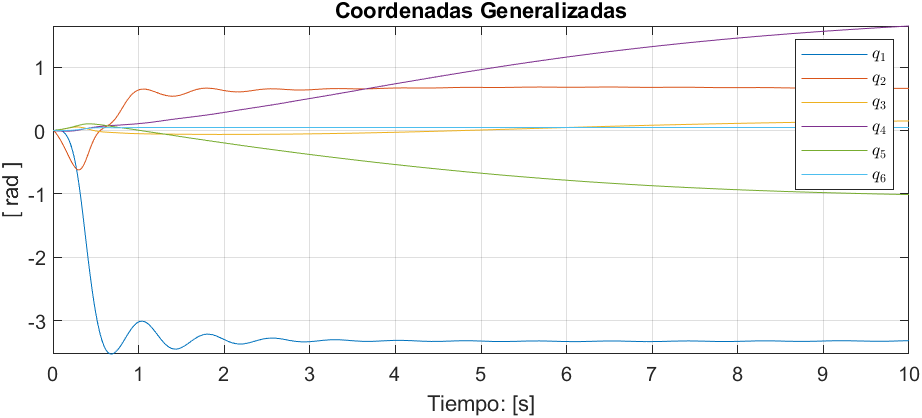
\includegraphics[scale=0.5]{coor_gen_caso_1.png} 
        \caption{Coordenadas Generalizadas Caso 1}
        \label{fig:CoordGenC1}
    \end{figure}

    \subsubsection{Velocidad Generalizada}
    La gráfica \ref{fig:VelGenC1}, presenta un cambio notable en la velocidad 
    de las articulaciones $q_1$ y $q_2$, esto debido a que ambas conforman 
    las articulaciones base del robot, y por lo tanto permiten definir la dirección 
    de movimiento del resto de los referenciales. De esta forma se explican las 
    variaciones de velocidad significativas de las primeras dos articulaciones, 
    mientras que el resto, cuyos eslabones se mueven en función de los dos primeros 
    en una respuesta libre del sistema, muestran variaciones menores de velocidad.

    \begin{figure}[H]% [!ht]
            \centering
            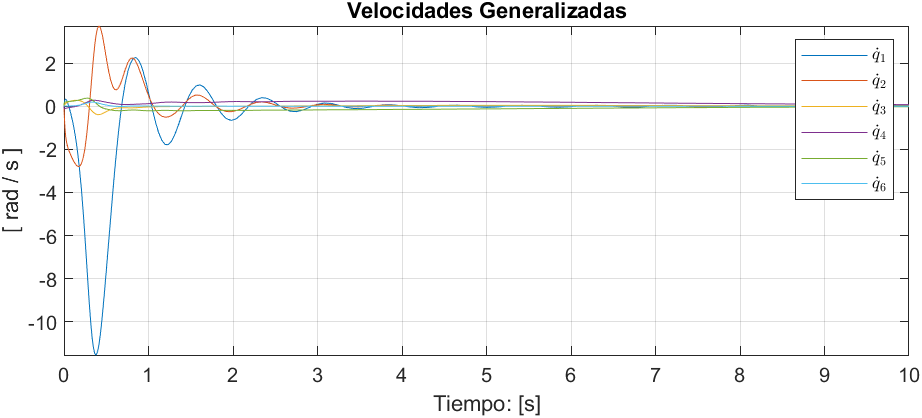
\includegraphics[scale=0.5]{vel_gen_caso_1.png} 
        \caption{Velocidad Generalizada Caso 1}
        \label{fig:VelGenC1}
    \end{figure}

    \subsubsection{Energía Cinética}

    En el caso de la figura \ref{fig:eCinC1} se identifica un pico en la energía 
    cinética a los 0.4 segundos y un punto de inflección hacia un estado estacionario 
    a partir del segundo 2, lo cual 
    es consistente con lo esperado, puesto que se observa una etapa de 
    amortiguamiento y pérdida de energía, hasta alcanzar el equilibrio. Esto significa 
    que cuando se suelta el exoesqueleto de su posición de \emph{Casa} y 
    empieze a moverse como un péndulo, llegará un instante en que se detenga el 
    movimiento oscilatorio, que es la fase de amortiguamiento observada.

    \begin{figure}[H]%[!ht]
            \centering
            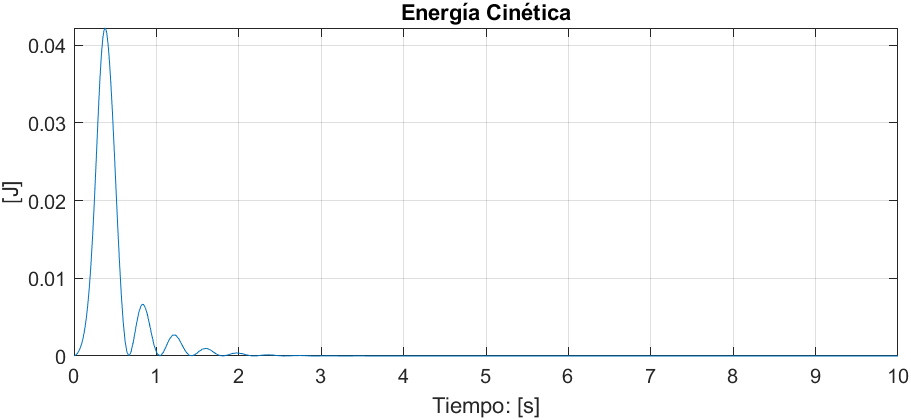
\includegraphics[scale=0.5]{ener_cin_caso_1.png} 
        \caption{Energía Cinética Caso 1}
        \label{fig:eCinC1}
    \end{figure}

    \subsubsection{Energía Potencial}
    La energía potencial inicia en 0.3 [J] y se puede observar en la figura 
    \ref{fig:ePotC1} que a partir del segundo 2 se llega a un punto de equilibrio al no tener 
    movimiento el exoesqueleto. Esto es consistente con los resultados obtenidos para 
    el rango máximo de la energía potencial, pues la misma o adquiere valores mayores al 
    inicial de la energía potencial, con lo cual se demuestra el efecto directo de las 
    fuerzas disipativas.

    \begin{figure} [H]%[!ht]
            \centering
            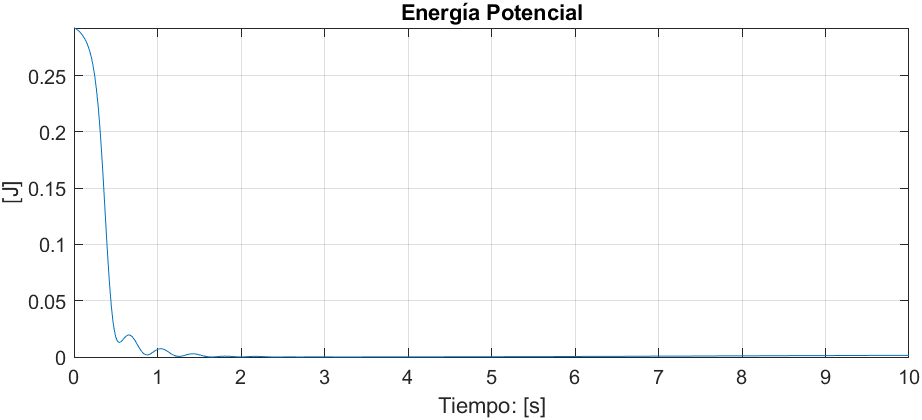
\includegraphics[scale=0.5]{ener_pot_caso_1.png} 
        \caption{Energía Potencial Caso 1}
        \label{fig:ePotC1}
    \end{figure}

    \subsubsection{Energía Mecánica}
    La energía mecánica es la suma de la energía cinética con la energía potencial. 
    la gráfica \ref{fig:eMecC1} resulta similar a la obtenida en \ref{fig:ePotC1} 
    debido a que la energía cinética presenta valores de una escala menor que los 
    obtenidos por la energía potencial, con lo cual es congruente que el comportamiento 
    del cambio de la energía mecánica dependa principalmente de este.

    \begin{figure} [H]%[!ht]
            \centering
            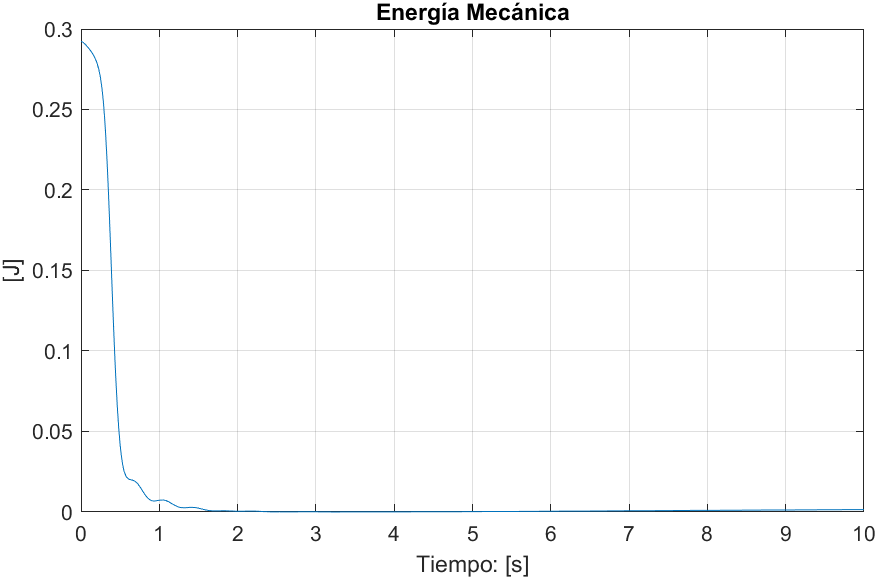
\includegraphics[scale=0.5]{ener_mec_caso_1.png} 
        \caption{Energía Mecánica Caso 1}
        \label{fig:eMecC1}
    \end{figure}

\subsection{Caso 2}\label{caso2}
    En el presente caso de estudio, se hicieron modificaciones en todos los 
    parámetros (torque, factor de disipación y tiempo de simulación), los 
    valores exactos se visualizan en la tabla \ref{ref:TablaC2}.

    \subsubsection{Parámetros} 
    \begin{table}[H]%[!ht]
        \centering
        \begin{center}
        \caption{Parámetros modificados del simulador (Sistema No Conservativo)} 
        \centering
        \bigskip
        \scalebox{0.7}{
            \begin{tabular}{c||cccccc|c}
            Parámetros & $\tau_1$ & $\tau_2$ & $\tau_3$ & $\tau_4$ & $\tau_5$ & $\tau_6$ & Unidades\\
            \hline
            Torques & -0.050 & 0.050 & -0.040 & -0.060 & 0.020 & 0.010 & [Nm] \\
            Factor de Disipación & \multicolumn{6}{c|}{0.006001} & [Ns/m] \\
            Tiempo de Simulación & \multicolumn{6}{c|}{20} & [s]\\
            \hline 
            \end{tabular}    }
        \end{center}
        \label{ref:TablaC2}
    \end{table}

    \subsubsection{Coordenadas Generalizadas}
    Las imágenes de la gráfica \ref{fig:CoordGenC2} son consistentes con los 
    valores dados en los torques, esto considerando que las fuerza aplicadas en las 
    articulaciones $q_1$, $q_3$ y $q_4$ se definieron con valores negativos,
    lo cual se ve representado en un giro en sentido negativo acorde a la regla 
    de la mano derecha.

    \begin{figure} [H]%[!ht]
            \centering
            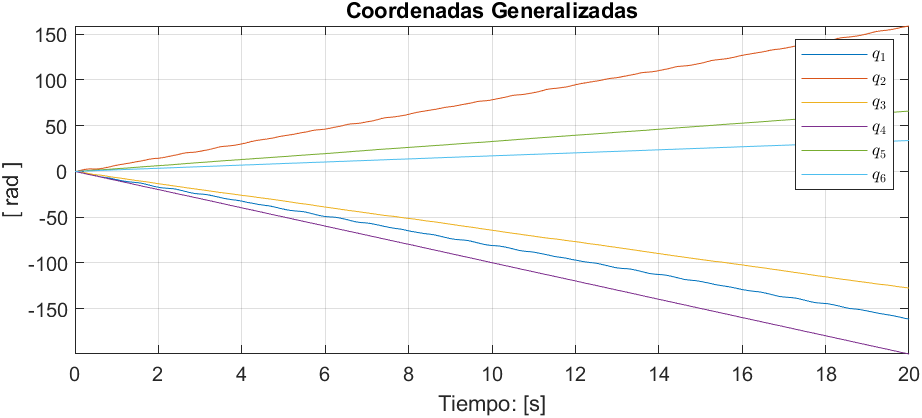
\includegraphics[scale=0.5]{coor_gen_caso_2.png} 
        \caption{Coordenadas Generalizadas Caso 2}
        \label{fig:CoordGenC2}
    \end{figure}

    \subsubsection{Velocidad Generalizada}
    Las articulaciones $q_1$ y $q_2$, en la gráfica \ref{fig:VelGenC2} 
    son las que presentan variaciones con una mayor amplitud de velocidad que el resto de 
    los valores de las velocidades generalizadas, 
    además se considera que las velocidades $\dot{q}_2$,$\dot{q}_5$ y 
    $\dot{q}_6$ toman valores positivos y esto es consistente con los torques aplicados.
    \begin{figure}[H]%[!ht]
            \centering
            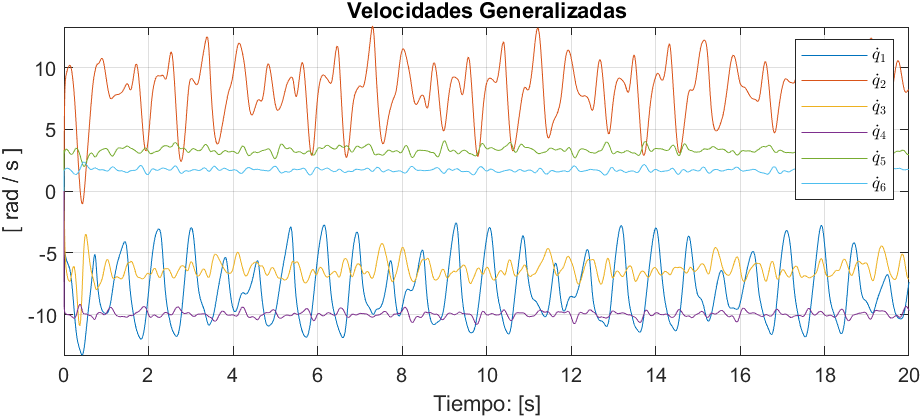
\includegraphics[scale=0.5]{vel_gen_caso_2.png} 
        \caption{Velocidad Generalizada Caso 2}
        \label{fig:VelGenC2}
    \end{figure}

    \subsubsection{Energía Cinética}
    La gráfica \ref{fig:eCinC2} demuestra una función periódica, la cual presenta valores 
    consistentes con el fenómeno físico que se observaría en el exoesqueleto al momento de 
    aplicar torques constantes, pues a diferencia del caso anterior en el que se presentaba 
    un punto de equilibrio, en este caso las articulaciones se encontrarían rotando de manera 
    permanente, con lo cual habría incrementos de energía cinética en todos los rangos en los que 
    se presente el giro en dirección al efecto de la fuerza de la gravedad, mientras que 
    la misma presentaría reducciones en el caso contrario.

    \begin{figure} [H]%[!ht]
            \centering
            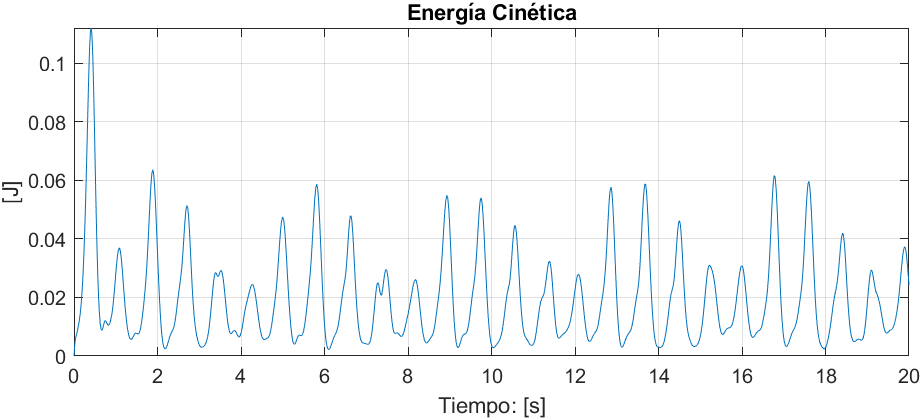
\includegraphics[scale=0.5]{ener_cin_caso_2.png} 
        \caption{Energía Cinética Caso 2}
        \label{fig:eCinC2}
    \end{figure}

    \subsubsection{Energía Potencial}
    La imagen obtenida por el osciloscopio, que se representa en la figura 
    \ref{fig:ePotC2}  muestra la periodicidad del movimiento que está teniendo 
    el exoesqueleto, algo importante a remarcar, es que está oscilando entre 
    los valores de 0[J] y 2.2[J], pero nunca llega a los mismos 3[J] de inicio, 
    debido a que posterior al estado base, el sistema no vuelve a tener todos 
    sus referenciales en la posición original. 
    
    Así mismo se observa que los puntos de energía potencial máxima, coinciden con 
    el inicio de los incrementos de energía cinética, con lo cual se refuerza la 
    idea del efecto de la fuerza de gravedad en relación a los incrementos y 
    decrementos de energía. 

    \begin{figure} [H]%[!ht]
            \centering
            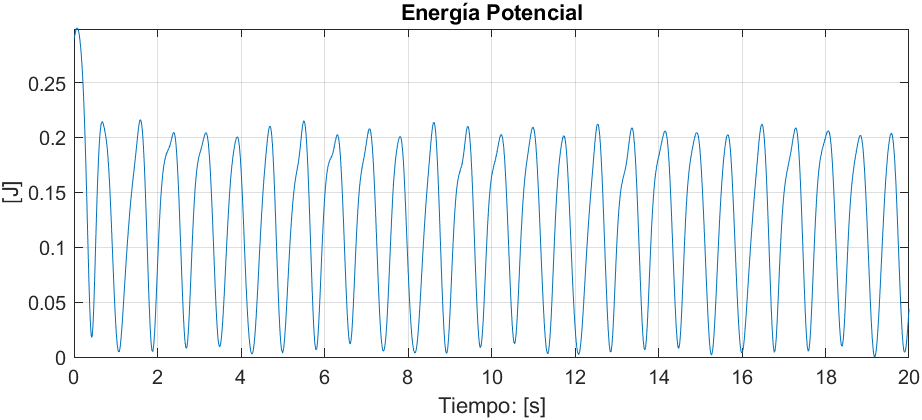
\includegraphics[scale=0.5]{ener_pot_caso_2.png} 
        \caption{Energía Potencial Caso 2}
        \label{fig:ePotC2}
    \end{figure}

    \subsubsection{Energía Mecánica}
    La gráfica de la figura \ref{fig:eMecC2} muestra un desfase positivo, 
    proporcional a la magnitud de la energía cinética, con respecto de la 
    gráfica de la figura \ref{fig:ePotC2}.
    \begin{figure} [H]%[!ht]
            \centering
            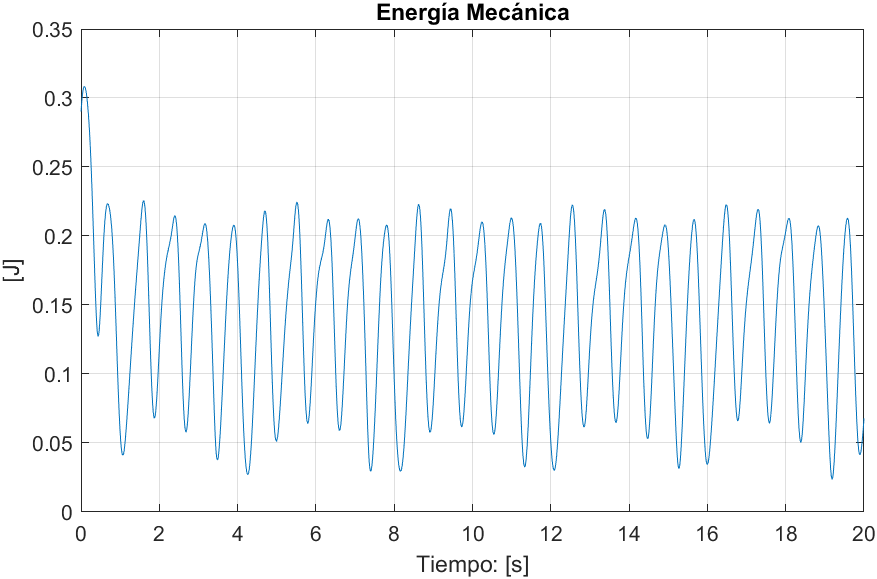
\includegraphics[scale=0.5]{ener_mec_caso_2.png} 
        \caption{Energía Mecánica Caso 2}
        \label{fig:eMecC2}
    \end{figure}

    

\subsection{Caso 3}\label{caso3}
    El último caso analizado representa un sistema conservativo, esto significa 
    un acercamiento a un sistema ideal donde no hay disipación de energía, 
    debido a que no se aplica una fuerza generada por una fricción viscosa.

    \subsubsection{Parámetros}

    Los parámetros que se utilizaron para el caso 3, se ven reflejados en la 
    tabla \ref{ref:TablaC3}, es decir, se están considerando torques nulos y 
    sin fricción, así mismo se incrementó el tiempo de simulación, para tener un 
    mayor espacio de muestreo en el análisis.

    \begin{table}[H]%[!ht]
        \centering
        \begin{center}
        \caption{Parámetros modificados del simulador (Sistema Conservativo)} 
        \centering
        \bigskip
        \scalebox{0.7}{
            \begin{tabular}{c||cccccc|c}
            Parámetros & $\tau_1$ & $\tau_2$ & $\tau_3$ & $\tau_4$ & $\tau_5$ & $\tau_6$ & Unidades\\
            \hline
            Torques & 0 & 0 & 0 & 0 & 0 & 0 & [Nm] \\
            Factor de Disipación & \multicolumn{6}{c|}{0} & [Ns/m] \\
            Tiempo de Simulación & \multicolumn{6}{c|}{200} & [s]\\
            \hline 
            \end{tabular}    }
        \end{center}
        \label{ref:TablaC3}
    \end{table}

    \subsubsection{Coordenadas Generalizadas}

    La gráfica \ref{fig:CoordGenC3} muestra los cambios en la posición 
    angular de cada una de las articulaciones a lo largo de 200 segundos 
    simulados, se aprecia que el 6to referencial $q_6$ es el que más rotaciones 
    presenta.

    \begin{figure} [H]% [!ht]
            \centering
            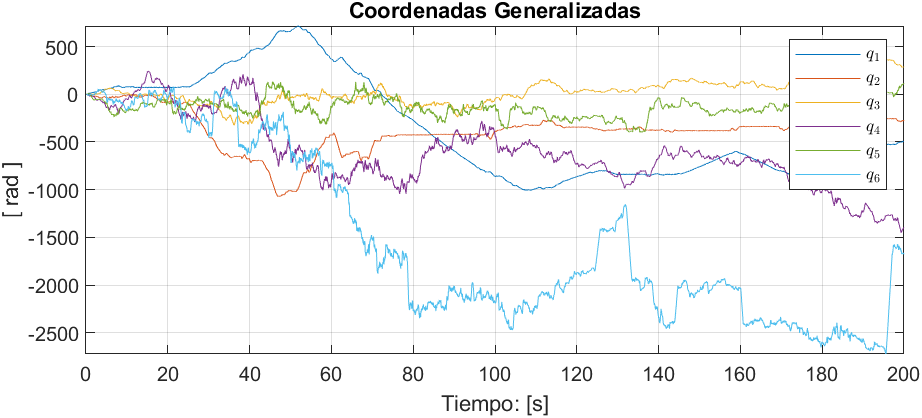
\includegraphics[scale=0.5]{coor_gen_caso_3.png} 
        \caption{Coordenadas Generalizadas Caso 3}
        \label{fig:CoordGenC3}
    \end{figure}

    \subsubsection{Velocidad Generalizada}

    La gráfica \ref{fig:VelGenC3} muestra en primer plano la velocidad 
    generalizada del referencial $q_6$ en azul claro, el cual en el espacio 
    de tiempo de 0 a 40 segundos presenta un incremento positivo en sus valores 
    absolutos de velocidad, alcanzando su punto máximo en el segundo 68, 
    a partir de ese momento empieza a disminuir su velocidad, para 
    finalmente estabilizar su valor en un rango de -1000 a 1000 
    rad/s, a partir de un tiempo de 120 segundos. 

    \begin{figure}[H]%[!ht]
            \centering
            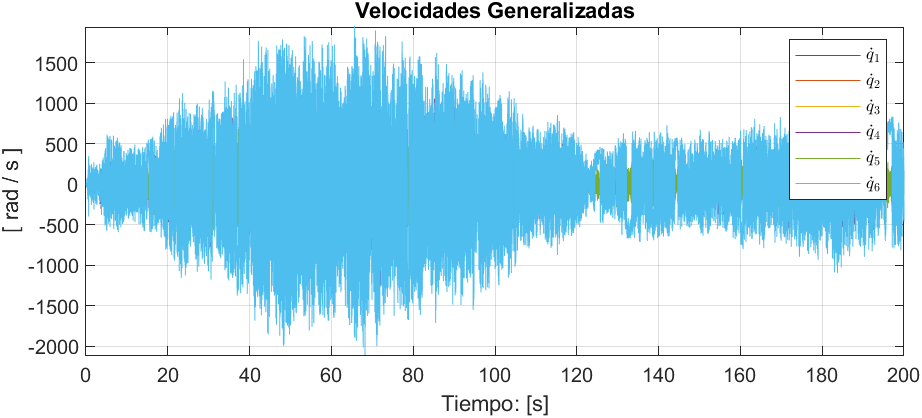
\includegraphics[scale=0.5]{vel_gen_caso_3.png} 
        \caption{Velocidad Generalizada Caso 3}
        \label{fig:VelGenC3}
    \end{figure}

    \subsubsection{Energía Cinética}

    La energía cinética representada en la gráfica \ref{fig:eCinC3} muestra 
    un pico a los 68 segundos, para finalmente tener un rango definido entre 
    0 y 1 Joule a partir de los 120 segundos.

    \begin{figure} [H]%[!ht]
            \centering
            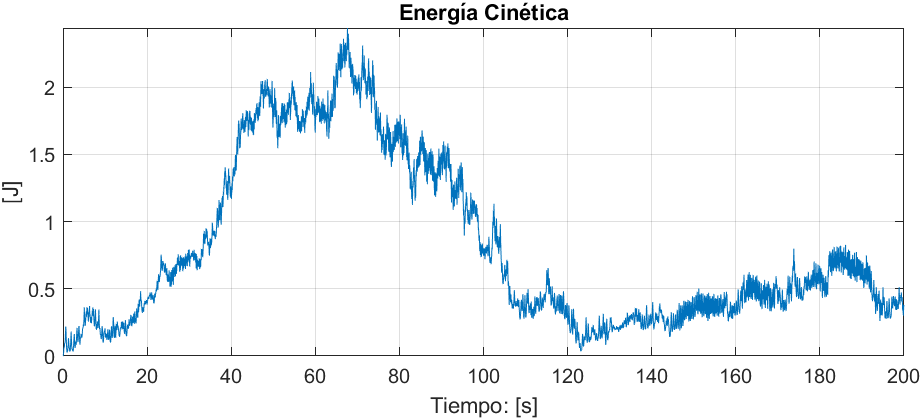
\includegraphics[scale=0.5]{ener_cin_caso_3.png} 
        \caption{Energía Cinética Caso 3}
        \label{fig:eCinC3}
    \end{figure}

    \subsubsection{Energía Potencial}

    La energía potencial es proporcional a la posición que tiene la cadena 
    cinemática en función a un "datum", debido a lo anterior la gráfica 
    \ref{fig:ePotC3} muestra que el exoesqueleto está tomando en promedio 
    valores constantes y cercanos a cero, por eso su rango está entre 0 y 
    0.3 [J], porqué está teniendo una rotación en un movimiento perpetuo, 
    al no haber fricción.

    \begin{figure} [H]%[!ht]
            \centering
            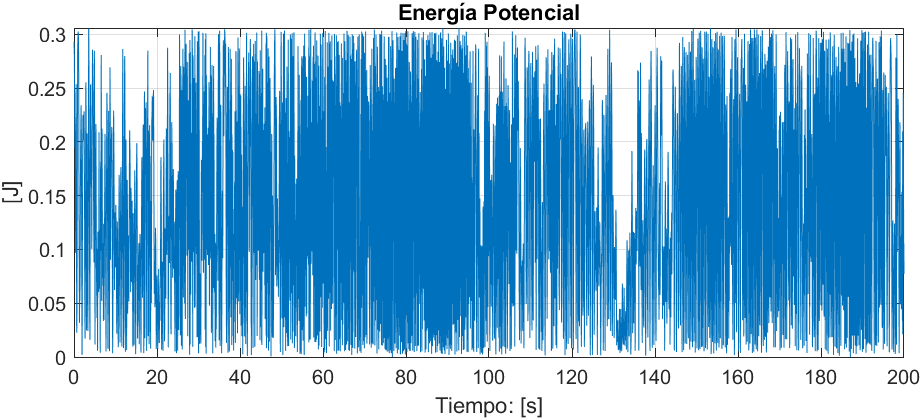
\includegraphics[scale=0.5]{ener_pot_caso_3.png} 
        \caption{Energía Potencial Caso 3}
        \label{fig:ePotC3}
    \end{figure}

    \subsubsection{Energía Mecánica}

    La gráfica \ref{fig:eMecC3} representa la energía mecánica total de 
    un sistema conservativo, cuyo valor máximo positivo es de 0.3 [J], puesto 
    que ese es el rango promedio máximo constante de la energía potencial. 
    El pico que se observa en el lapso del tiempo de 0 a 68 segundos 
    refleja una inconsistencia a las leyes de la termodinámica, debido 
    a que está reflejando creación de energía cinética, pues supera el 
    rango máximo de la energía potencial.

    \begin{figure}[H]%[!ht]
            \centering
            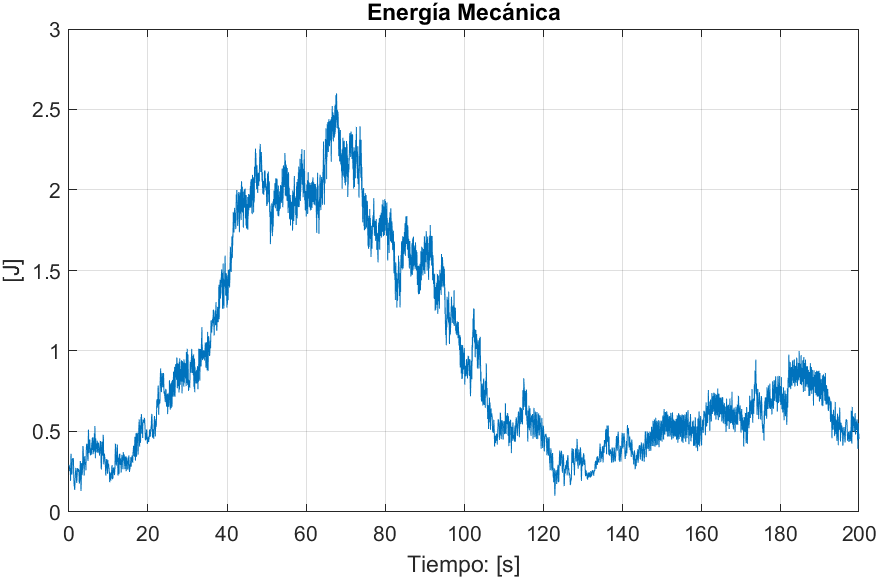
\includegraphics[scale=0.5]{ener_mec_caso_3.png} 
        \caption{Energía Mecánica Caso 3}
        \label{fig:eMecC3}
    \end{figure}